\section{Results}
\subsection{Audit results}
\label{sec:audit}
Table~\ref{tab:data} summarizes the cleaning. ISOT lost 5,762 exact duplicates (12.8\% of its 44,898 rows) and WELFake 8,601 (11.9\%). All 38,030 cleaned ISOT documents and all 6,005 cleaned McIntire documents have a normalized exact-text match in WELFake, whereas ISOT and McIntire share only 2 exact and about 33 near-duplicate documents (0.1\% and 0.5\%). WELFake is therefore not an independent third dataset, and we speak of three analysis corpora derived from three public datasets. The residual corpus contains 17,162 documents (10,427 real and 6,735 fake) and is used as the third analysis corpus. Fig.~\ref{fig:overlap} summarizes the construction.

\begin{figure}[t]
\centering
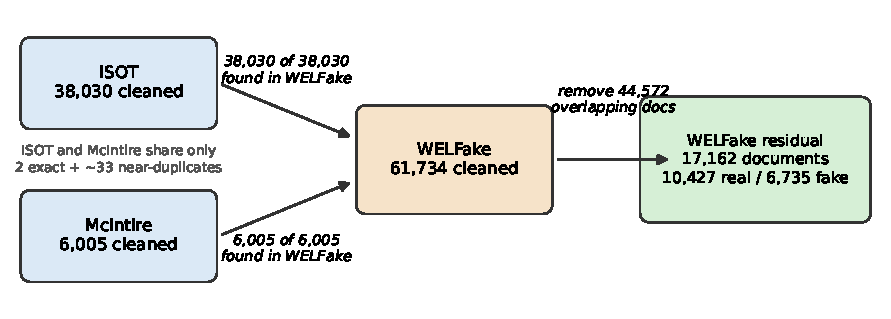
\includegraphics[width=0.86\textwidth]{fig_overlap.pdf}
\caption{Construction of the WELFake residual. Every cleaned ISOT and McIntire document has a normalized exact-text match in WELFake; ISOT and McIntire share almost no documents. WELFake documents flagged by the builder's stripped-body exact, prefix or primary near-duplicate rules are removed to leave the residual used as the third dataset. One stripped-empty exact match survives this policy, as described in the methods.}
\label{fig:overlap}
\end{figure}

\begin{table}[t]
\caption{Datasets. Raw and cleaned sizes, and the analysis set (real/fake).}
\label{tab:data}
\centering\footnotesize\setlength{\tabcolsep}{3pt}
\adjustbox{max width=\linewidth}{\begin{tabular}{@{}lrrrr@{}}
\toprule
Dataset & Raw & Cleaned & Analysis set (R/F) & Mean words (R/F)\\
\midrule
ISOT & 44,898 & 38,030 & 20,923/17,107 & 395/448\\
McIntire & 6,335 & 6,005 & 2,964/3,041 & 939/709\\
WELFake residual & 72,134 & 61,734 & 10,427/6,735 & 895/640\\
\bottomrule
\end{tabular}}
\par\vspace{2pt}\begin{minipage}{0.97\columnwidth}\scriptsize\raggedright Cleaning removed short/empty documents (1,106; 211; 1,799) and exact duplicates (5,762; 119; 8,601). Raw and cleaned sizes for the WELFake row refer to the full corpus; its analysis set is the residual, which excludes 44,572 documents that overlap ISOT or McIntire. Mean words are for title plus body.\end{minipage}
\end{table}


\subsection{Document-paired validation}\label{sec:paired}
The main intervention estimates below use the new document-paired protocol, rather than the archived condition-specific samples. All eight seeds (0--7) completed: 312 TF-IDF fits and 192 fits for each transformer, producing 2,088 evaluation rows (each fit evaluated on its own and the other two corpora). Article-selection manifests agree across all three models. Within each seed, corpus and length-matching setting, masking conditions and their random controls reuse identical training and evaluation articles. Cluster separation, sample counts and hashes passed the saved-provenance audit. This validates result completeness and recorded pairing; it does not independently repeat training, NER or the raw-text overlap audit.

\paragraph{TF-IDF: the main finding persists.}
The pooled baseline AUC gap is 0.212, falling to 0.157 under S+L+E (Table~\ref{tab:paired_conditions}). The seed-wise share removed is 26.2\% (95\% interval 24.5--27.8\%), compared with 24.7\% in the archived run. L+E alone removes 27.5\% (25.7--29.2\%). Adding source-marker masking does not increase this raw reduction; its negative matched-control contrast is consistent with the slightly smaller S+L+E reduction, without identifying a unique mechanism. These percentages are calculated within seed before averaging, not from rounded pooled gaps. Length matching raises cross-dataset AUC by 0.037 [0.033, 0.040]. Entity masking exceeds matched random deletion by 0.021 [0.019, 0.023], and retains its advantage after length matching: 0.021 [0.020, 0.022]. S+L+E exceeds its length-matched random control by 0.013 [0.012, 0.015]. All four pooled contrasts have the same sign in eight of eight seeds. Source masking falls below its random control by 0.009 [0.009, 0.010]; it does not account for the positive combined result.

\begin{table}[t]
\caption{Document-paired validation: pooled cross-dataset AUC and AUC gap (mean and 95\% interval over eight seeds). Six ordered pairs are averaged within seed.}\label{tab:paired_conditions}
\centering\footnotesize
\adjustbox{max width=\linewidth}{\begin{tabular}{@{}llcc@{}}
\toprule
Model & Condition & Cross AUC & AUC gap\\
\midrule
TF-IDF & C0 & 0.772 [0.768, 0.777] & 0.212 [0.208, 0.217]\\
TF-IDF & L+E & 0.825 [0.821, 0.830] & 0.154 [0.151, 0.157]\\
TF-IDF & S+L+E & 0.816 [0.811, 0.821] & 0.157 [0.154, 0.160]\\
TF-IDF & L+$R_E$ & 0.804 [0.800, 0.809] & 0.179 [0.176, 0.182]\\
TF-IDF & L+$R_{SE}$ & 0.803 [0.799, 0.808] & 0.180 [0.177, 0.184]\\
DistilBERT & C0 & 0.813 [0.791, 0.836] & 0.184 [0.161, 0.207]\\
DistilBERT & L+E & 0.828 [0.821, 0.835] & 0.167 [0.160, 0.174]\\
DistilBERT & S+L+E & 0.834 [0.827, 0.842] & 0.158 [0.150, 0.166]\\
DistilBERT & L+$R_E$ & 0.841 [0.832, 0.850] & 0.155 [0.147, 0.164]\\
DistilBERT & L+$R_{SE}$ & 0.842 [0.834, 0.850] & 0.154 [0.146, 0.162]\\
RoBERTa & C0 & 0.812 [0.776, 0.847] & 0.188 [0.152, 0.224]\\
RoBERTa & L+E & 0.902 [0.892, 0.913] & 0.096 [0.085, 0.107]\\
RoBERTa & S+L+E & 0.910 [0.902, 0.918] & 0.088 [0.079, 0.096]\\
RoBERTa & L+$R_E$ & 0.916 [0.908, 0.923] & 0.083 [0.076, 0.091]\\
RoBERTa & L+$R_{SE}$ & 0.900 [0.887, 0.913] & 0.099 [0.086, 0.112]\\
\bottomrule
\end{tabular}
}
\end{table}

\paragraph{Transformers: raw gains do not isolate a cue effect.}
DistilBERT entity masking performs worse than matched random deletion by 0.028 AUC [$-$0.039, $-$0.017], with negative differences in all eight seeds (Table~\ref{tab:paired_pooled}). This is clearer than the archived estimate of $-0.010$ [$-$0.025, 0.005]. With length matching the difference is $-0.013$ [$-$0.020, $-$0.005], but it does not survive the descriptive six-contrast Holm adjustment. For S+L+E the DistilBERT estimate is $-0.007$ [$-$0.018, 0.003], and for RoBERTa it is $+0.010$ [$-$0.010, 0.030]; both intervals include zero. Neither establishes equivalence. RoBERTa's E and L+E contrasts also have intervals spanning zero.

RoBERTa's S+L+E gap falls from 0.188 to 0.088, a seed-wise raw reduction of 50.8\% [39.5, 62.2\%]. Its length-matched random control already has a gap of 0.099 and cross-dataset AUC of 0.900, against 0.910 for S+L+E. Thus a large raw reduction does not establish a benefit specific to the selected cues. The focused transformer validation did not include S, S+E, $R_S$ or $R_{SE}$, so the archived $+0.102$ RoBERTa random-deletion result was not directly retested. The validation supports sensitivity to random deletion through the tested controls, rather than reproducing that exact contrast.

\begin{table}[t]
\caption{All six document-paired cross-dataset AUC contrasts in the descriptive multiplicity family: mean and 95\% interval over eight seeds. Positive values favor the first condition. L versus C0 changes article selection by design; masking comparisons within each length setting reuse identical articles. ``Not run denotes an omitted transformer contrast, assigned $p=1$ only for multiplicity adjustment (Table~\ref{tab:paired_multiplicity}).}\label{tab:paired_pooled}
\centering\scriptsize
\adjustbox{max width=\linewidth}{\begin{tabular}{@{}lccc@{}}
\toprule
Contrast & TF-IDF & DistilBERT & RoBERTa\\
\midrule
S $-$ $R_S$ & -0.009 [-0.010, -0.009] & not run & not run\\
E $-$ $R_E$ & +0.021 [+0.019, +0.023] & -0.028 [-0.039, -0.017] & -0.009 [-0.024, +0.007]\\
S+E $-$ $R_{SE}$ & +0.012 [+0.010, +0.013] & not run & not run\\
L $-$ C0 & +0.037 [+0.033, +0.040] & +0.016 [-0.003, +0.035] & -0.006 [-0.032, +0.020]\\
L+E $-$ L+$R_E$ & +0.021 [+0.020, +0.022] & -0.013 [-0.020, -0.005] & -0.013 [-0.029, +0.003]\\
S+L+E $-$ L+$R_{SE}$ & +0.013 [+0.012, +0.015] & -0.007 [-0.018, +0.003] & +0.010 [-0.010, +0.030]\\
\bottomrule
\end{tabular}
}
\end{table}

\begin{figure}[t]
\centering
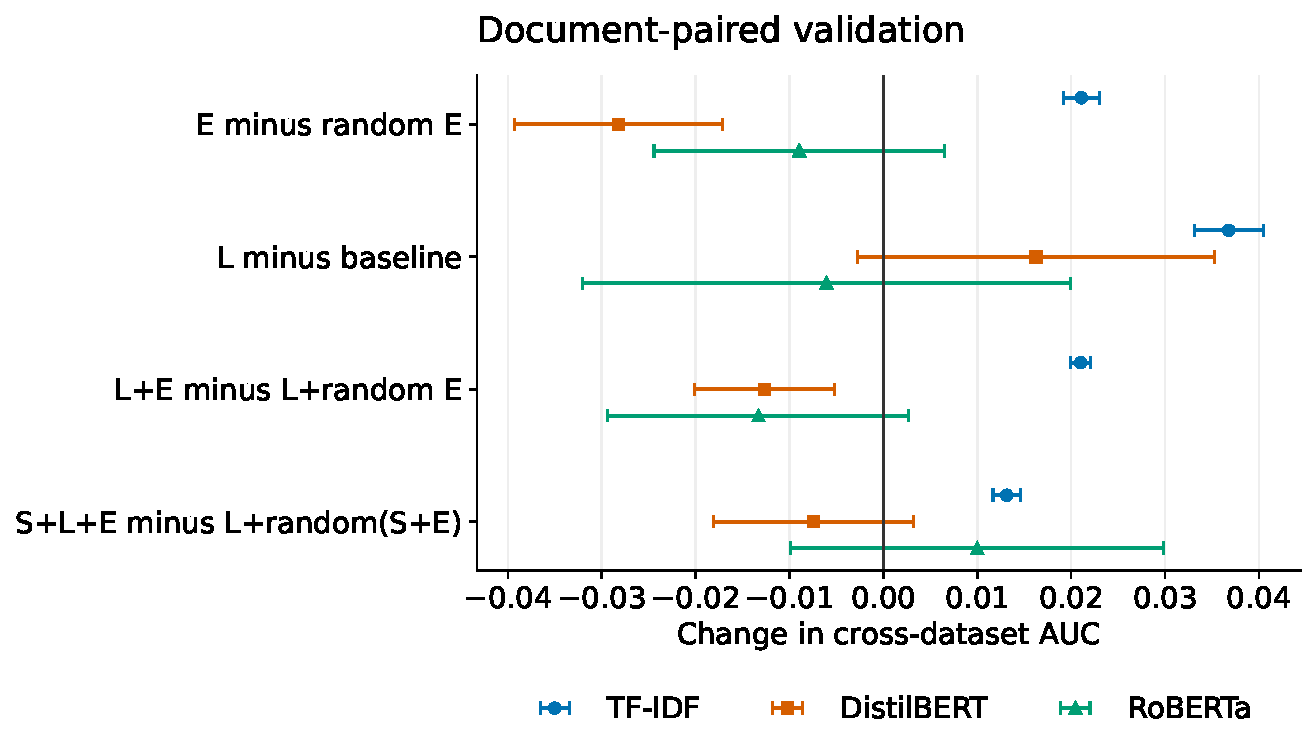
\includegraphics[width=\linewidth]{paired_validation_contrasts.pdf}
\caption{Document-paired pooled contrasts. Points and bars show means and 95\% intervals over eight seeds; the six ordered pairs are averaged within each seed. Intervals describe variability on these fixed corpora.}\label{fig:paired}
\end{figure}

\paragraph{Model differences.}
Direct seed-wise differences support a larger entity-specific effect for TF-IDF than DistilBERT: E against $R_E$ differs by 0.049 [0.038, 0.060], and L+E against L+$R_E$ differs by 0.034 [0.026, 0.041]. These model-difference estimates are descriptive and are reported in the supplement with seed values. Matching document identities across models does not make the models' optimization randomness identical.

\paragraph{Dataset-pair variation.}
Table~\ref{tab:paired_pairs} reports S+L+E against its length-matched random control. For DistilBERT, McIntire$\rightarrow$ISOT is positive (0.101 [0.074, 0.129]), all four residual-involving transfers are negative with intervals below zero, and ISOT$\rightarrow$McIntire is positive but its interval narrowly includes zero (0.028 [$-$0.0001, 0.056]). For RoBERTa, both ISOT--McIntire transfers have positive intervals, but ISOT$\rightarrow$residual is highly uncertain (0.046 [$-$0.056, 0.148]); only residual$\rightarrow$McIntire is clearly negative by its unadjusted interval. The archived claim that both transformers consistently lose against the control on residual-involving transfers is therefore not supported by the paired run. TF-IDF benefits on all four ISOT-involving transfers, whereas the McIntire--residual transfers are negative. All pair-level intervals are exploratory and unadjusted.

\begin{table}[t]
\caption{Document-paired S+L+E minus L+$R_{SE}$ by ordered pair: mean and 95\% interval over eight seeds. Exploratory; no pair-level multiplicity correction. ``Residual'' is the constructed WELFake residual.}\label{tab:paired_pairs}
\centering\scriptsize
\adjustbox{max width=\linewidth}{\begin{tabular}{@{}lccc@{}}
\toprule
Train $\rightarrow$ test & TF-IDF & DistilBERT & RoBERTa\\
\midrule
ISOT$\rightarrow$McIntire & +0.013 [+0.011, +0.015] & +0.028 [-0.000, +0.056] & +0.028 [+0.007, +0.049]\\
ISOT$\rightarrow$residual & +0.004 [+0.001, +0.007] & -0.050 [-0.075, -0.025] & +0.046 [-0.056, +0.148]\\
McIntire$\rightarrow$ISOT & +0.058 [+0.053, +0.064] & +0.101 [+0.074, +0.129] & +0.028 [+0.002, +0.054]\\
McIntire$\rightarrow$residual & -0.009 [-0.012, -0.007] & -0.017 [-0.027, -0.006] & -0.012 [-0.025, +0.001]\\
residual$\rightarrow$ISOT & +0.021 [+0.015, +0.027] & -0.077 [-0.115, -0.039] & -0.014 [-0.030, +0.002]\\
residual$\rightarrow$McIntire & -0.009 [-0.011, -0.006] & -0.031 [-0.045, -0.017] & -0.016 [-0.025, -0.006]\\
\bottomrule
\end{tabular}
}
\end{table}

\paragraph{Multiplicity and comparison with archived results.}
All six TF-IDF contrasts in the descriptive family have exact sign-flip $p=0.0078$ and Holm-adjusted $p=0.0469$. DistilBERT's E against $R_E$ has the same adjusted value; its other tested contrasts and all RoBERTa contrasts have adjusted values above 0.05. Table~\ref{tab:paired_multiplicity} lists all six contrasts, sign agreement, exact and adjusted values, including the omitted transformer contrasts assigned $p=1$. These are descriptive sensitivity summaries: the protocol was written after the original findings were known, and the seeds reuse one fixed document universe. The new run is not an independent-corpus replication or a registered confirmatory test. Archived and paired estimates are tabulated separately in the supplement. Their differences include changed sampling and recorded software versions; they cannot be attributed solely to document pairing. Appendix~\ref{sec:archived} preserves the archived factorial, exploratory and duplicate-removal results, which were not all repeated in the focused validation.
